% main.tex
\documentclass[12pt]{article}

\usepackage[margin=1in]{geometry}
\usepackage{natbib}
\usepackage{hyperref}
\hypersetup{
  colorlinks=true,
  linkcolor=blue,
  filecolor=magenta,
  citecolor=blue,
  urlcolor=cyan,
  pdftitle={How to Study Boundary Phenomena},
  pdfpagemode=FullScreen,
}
\usepackage[T1]{fontenc}
\usepackage[utf8]{inputenc}
\usepackage{amsmath}
\usepackage{graphicx}
\usepackage{tipa}
\usepackage{setspace}
\usepackage{booktabs}
\usepackage{ulem}
\usepackage{csquotes}
\usepackage{linguex}


\title{Language as a Stack of Homeostatic Property-Cluster Kinds: From Phonemes to Constructions}
\author{Brett Reynolds}
\date{}

\begin{document}
\maketitle
\doublespacing

\begin{abstract}
\noindent Language categories must be stable enough for communication yet flexible enough to change over time. Many linguistic categories~-- from phonemes to words to grammatical constructions~-- maintain this balance through what philosophers of science call \textsc{homeostatic property clusters}: groups of co-occurring features held together not by fixed essences but by identifiable mechanisms. This paper develops an operational test for when a linguistic category qualifies as such a cluster. 

I propose two diagnostics. First, \textsc{projectibility}: the category must support reliable prediction about new data. Second, \textsc{homeostasis}: specific mechanisms must demonstrably maintain the cluster's coherence. I apply these tests at three levels of linguistic structure. For phonemes, I show that inventory sizes cluster in a 20–50 segment band across language families, and that marked vowels like /y/ become more probable as vowel systems grow~-- patterns maintained by articulatory constraints, perceptual learning, and social norms. For words, I track how \textit{egregious} shifts meaning over decades while preserving enough distributional coherence that models trained on earlier usage can still identify it later. For constructions, I demonstrate that English \textit{let alone} \citep{FillmoreKayOConnor1988} maintains a stable bundle of cues (the phrase itself, syntactic parallelism, scalar/downward-entailing licensing) that projects across different text collections.

Equally important are the failures: nonce words lack stabilizing mechanisms; cross-linguistic categories like "resultative" pool heterogeneous local mechanisms; complement classes defined by what they exclude have no positive cluster to maintain. These boundaries prevent over-application of the framework.

The contribution is methodological: concrete, reproducible tests for deciding when a linguistic category earns treatment as a stable kind. The approach remains neutral about grammatical frameworks~-- it asks what patterns travel and why, not how to represent them theoretically. Where categories pass both diagnostics, we gain principled grounds for their cognitive reality. Where they fail, we learn something about the limits of linguistic generalization.
\end{abstract}

\section{Introduction}
Language presents a familiar problem for cognitive science: the categories we rely on to speak and understand are stable enough to underwrite reliable inference but flexible enough to drift and diversify. Consider how the phoneme /r/ varies across English dialects but remains recognizable, or how the word \textit{awful} drifted from `awe-inspiring' to `terrible' while keeping its identity. An attractive middle ground for understanding such categories~-- originating in Boyd's account of \textsc{homeostatic property-cluster} (HPC) kinds~-- offers a way to reconcile stability with change \citep{Boyd1991Enthusiasm,Boyd1999Homeostasis}\footnote{For the first explicit HPC formulation (applied to moral terms), see \citet[§3.8]{Boyd1988MoralRealist}. For an explicit allowance that social mechanisms can underwrite homeostasis, see \citet{Boyd2000Workmanship}.}.

Such kinds emerge when identifiable forces keep characteristic features bundled~-- not through essence, but through contingent regularities. The category holds together as a family of properties maintained by mechanisms (biophysical, developmental, social) strongly enough to support induction. Think of biological species: robins share characteristic features~-- size, coloration, song patterns, nesting behavior~-- not because of an essential `robin-ness' but because developmental programs, ecological pressures, and reproductive isolation keep these traits correlated generation after generation. Boyd's insight is that many scientific and social categories work similarly: they are probabilistic clusters stabilized by mechanisms that keep enough of the cluster together for inductive use. 

This article proposes a general, testable program: many linguistic categories~-- phonemes, lexemes, and language-internal constructions~-- are HPC kinds. The claim is operational, not merely analogical. I test the claim with two simple diagnostics that any proposed linguistic category must pass. First, \textsc{Projectibility}: tokens must support reliable out-of-sample inference about form, meaning, or distribution. Second, \textsc{Homeostasis}: the property cluster must be tied to specific stabilizers with demonstrable covariance. I apply these diagnostics across levels with compact, reproducible case studies, alongside a principled failure taxonomy that blocks over-generalization. On this understanding, I treat phonemes, words, and language-internal constructions (e.g., English \textit{let alone}) as a posteriori kinds maintained by identifiable stabilizers.

For words, \citet{Miller2021WordsSpeciesKinds} develops this stance, rejecting essence-based individuation in favor of mechanism-indexed clusters that are historically delimited and population-relative. On this view, word-kinds earn their status because internal (cognitive) and external (normative) mechanisms sustain covarying properties~-- pronunciation, orthography, meaning, distribution~-- so that speakers can project from attested tokens to new ones. The word \textit{dog}, for instance, maintains its identity not through a platonic essence but because spelling conventions, pronunciation norms, semantic associations, and syntactic patterns travel together, stabilized by frequency of use, literacy education, and community practice.

At the phonological level, recent work by \citet{Ekstrom2025PhonemeTool} argues that phonemes are culturally maintained \textsc{cognitive tools} anchored in articulatory and auditory constraints. Two quantitative signatures exemplify the sort of measurable \enquote{homeostasis} HPC requires: family-wise \textsc{ridgelines} of inventory sizes (showing most languages cluster roughly between 20 and 50 segments across unrelated language families; see Figure \ref{fig:ridgelines}), and a scaling curve in which the probability that a language includes /y/ rises with vowel-inventory size, while /i/ remains common even in small systems.

Both patterns are presented with explicit methodological detail and tied to biophysical and efficiency pressures, drawing on data from PHOIBLE, an openly available database of segmental phoneme inventories for over 2{,}000 languages worldwide \citep{MoranEtAl2019PHOIBLE}, and a compact checklist of tool criteria summarizes the stabilizers involved \citep[Fig.\,1 p.\,4; Fig.\,2 p.\,7; Table\,1 p.\,14]{Ekstrom2025PhonemeTool}. These are precisely the ingredients HPC seeks: projectible distributions and identifiable stabilizing mechanisms.

The first case study revisits the phoneme level using the PHOIBLE database introduced above, but focuses on observable patterns rather than re-deriving articulatory physiology. I examine two signatures: how inventory sizes cluster by language family (visualized as ridgelines), and how the probability of finding /y/ in a language increases with the size of its vowel inventory. These patterns survive robustness checks like sampling one language per subfamily. The HPC reading is straightforward: the tight clustering within families demonstrates projectibility (new languages behave like their relatives), while the known mechanisms~-- quantal stability, dispersion, developmental tuning, and community norms~-- provide the homeostatic foundation.

The second case study turns to words. Building on \citet{Miller2021WordsSpeciesKinds}, I track how a single lexeme's meaning changes over time (e.g., how \textit{awful} drifted from positive to negative) while examining whether its contextual patterns~-- what words appear near it~-- remain coherent enough that a model trained on earlier decades can still identify the word in later ones. This demonstrates projectibility empirically. The homeostasis comes from multiple forces: entrenchment through repeated use and norm-guided conventions ensure that even as meanings shift, the word's spelling, pronunciation, and core distributional patterns stay bundled together at usable levels.

The third case study treats an English construction, \textit{let alone} \citep{FillmoreKayOConnor1988}, as a language-internal HPC kind. This construction (as in \textit{I can't afford coffee, \uline{let alone} dinner}) signals that the second item is even less likely than the first. Its identifying features~-- the phrase itself, parallel syntax between the contrasted items, and negative context~-- work together as a cue bundle that remains stable across different text collections. I test projectibility by training a model to recognize the construction in one corpus and seeing if it succeeds in another. The stabilizers that maintain this pattern include its frequency of use, the redundancy of its multiple cues (if one fails, others compensate), and normative enforcement through editorial practices that correct malformed instances.

Equally important are the failure cases~-- categories that don't qualify as HPC kinds. Some proposals are too thin: one-off items (like nonce coinages such as \textit{bromance} before it caught on), speech errors that blend words together, and children's overregularizations (\textit{goed} for `went') lack the stabilizers that would make them predictable beyond their immediate context. Others are too fat: when typologists group together all \enquote{resultative} constructions across languages, or all \enquote{ditransitive} patterns, they're pooling structures maintained by completely different mechanisms in each language \citep{Haspelmath2010}. Since the stabilizing mechanisms are local to each language, the cross-linguistic umbrella isn't a single HPC kind. Finally, negative or complement classes (e.g., \enquote{all ungrammatical strings}) are defined by what they're not, rather than by shared properties held together by identifiable mechanisms. The discipline here is mechanism-first, in line with the word-kinds program \citep{Miller2021WordsSpeciesKinds}.

The framework yields predictions and disconfirmers. A perturbation prediction: weakening a stabilizer (e.g., lowering frequency or impoverishing input) will reduce cluster covariance before norms re-stabilize~-- a pattern testable under register shifts or in learner corpora. A scaling prediction: rarer but quantally robust members (e.g., /y/ in the vowel space) become more probable as system size grows; analogously, low-frequency constructional variants should be more prevalent in larger constructicons. Both predictions borrow directly from the phoneme results \citep[Fig.\,2 p.\,7]{Ekstrom2025PhonemeTool} and extend them to higher levels.

In sum, properly operationalized HPC naturalizes linguistic ontology for cognitive science. It tells us when a category is the right sort of thing to underwrite inference, what keeps it stable enough, and how it can change. At the phoneme level, the ridgeline and scaling patterns already instantiate homeostasis under constraint; at the word and construction levels, analogous signatures can be demonstrated with standard corpus methods. The result isn't that everything is an HPC, but that many linguistic categories pass a disciplined test~-- and some don't \citep{Miller2021WordsSpeciesKinds,Ekstrom2025PhonemeTool}.

\section{Framework and diagnostics}\label{sec:framework}

The introduction outlined how linguistic categories might qualify as homeostatic property-cluster kinds. This section operationalizes that claim into executable diagnostics with specific thresholds and falsifiable predictions.

The two diagnostics~-- projectibility and homeostasis~-- require different evidence at each linguistic level:

Projectibility: Can we predict new data from old? If phonemes form genuine kinds, then knowing a language's family should constrain expectations about its inventory size. If words are kinds despite semantic drift, then patterns learned from earlier decades should help identify the same word later. If constructions are kinds, then cue patterns from one corpus should work in another. By contrast, nonce words or one-off blends would fail this test~-- they lack the regularities that enable prediction. This isn't philosophical hand-waving~-- it means concrete metrics like cross-validated prediction accuracy and held-out F1 scores.

Homeostasis: What keeps the patterns stable? The term \enquote{homeostasis} captures how mechanisms actively maintain property clusters despite perturbations, analogous to biological self-regulation. For each category, I name specific mechanisms and look for their signatures. Phonemes are stabilized by quantal regions that create articulatory \enquote{sweet spots} \citep{Stevens1989Quantal}, dispersion that maintains distinctiveness \citep{LiljencrantsLindblom1972}, perceptual magnets that pull varied pronunciations toward prototypes \citep{KuhlEtAl1991}, and community norms that transmit systems across generations. These mechanisms predict specific patterns: languages should converge on similar inventory sizes (not scatter randomly), and marked vowels like /y/ should appear mainly in larger systems (not randomly).

The protocol is straightforward: identify clustered properties, name stabilizers, test prediction, verify signatures. Where both tests succeed, the category qualifies as an HPC kind for that population and time period. Where they fail~-- no predictive power or no credible mechanisms~-- the category might be useful for description but doesn't constitute a kind in this technical sense. Section 6 details the failure modes: categories that are too thin, too fat, or merely negative complement classes.

Recent work provides models for what success looks like. Phonemes show remarkably consistent inventory sizes across language families and systematic scaling patterns for marked segments~-- exactly what we'd expect from the mechanisms described above \citep{Ekstrom2025PhonemeTool}. Words maintain enough coherence through meaning change that their identifying features~-- spelling, pronunciation, distribution~-- stay bundled at usable levels \citep{Miller2021WordsSpeciesKinds}.

Two constraints prevent overreach. First, claims are local: a category might be an HPC kind in one language or time period but not another. Cross-linguistic categories like \enquote{resultative} often pool constructions maintained by completely different mechanisms in each language~-- these are useful classifications but not single kinds. Second, negative categories don't qualify: \enquote{all ungrammatical strings} or \enquote{exceptions to rule R} are defined by what they lack, not by properties held together by mechanisms. The approach remains neutral about grammatical frameworks~-- it asks what patterns travel and why, not how to represent them theoretically.

\section{Methods: tests, scope, and robustness}\label{sec:methods}

The metaphysics is modest; the tests must be executable. This section outlines the conceptual approach and primary success criteria; complete statistical specifications appear in Appendix~A.

\subsection{Scope and populations}

Claims are local to specific populations and periods. Phoneme results apply to the PHOIBLE 2.0 snapshot as integrated with Glottolog/WALS for genealogy and area. Word results apply to contemporary written English in large, time-stamped corpora spanning the 20th--21st centuries. Construction results apply to UD-annotated English (news/web genres) in the 2010s--2020s. The program isn't a universal ontology of linguistic kinds; it is a method for deciding when a proposed category earns kindhood by passing predictive and mechanism-indexed tests.

\subsection{Executable diagnostics}

The two core diagnostics~-- projectibility and homeostasis~-- require different evidence at each linguistic level, but the logic remains constant: can patterns learned from one dataset predict another, and do identifiable mechanisms maintain those patterns?

\textit{Projectibility} tests whether categories support out-of-sample prediction. For phonemes, I ask whether vowel inventory size predicts the presence of marked segments like /\textipa{y}/~-- a front rounded vowel requiring precise articulatory coordination. Success requires a positive relationship (odds-ratio $>$1 with 95\% confidence), reasonable discrimination (10-fold cross-validated AUC $\geq$ 0.70), and monotonicity (verified by trend test at $\alpha = 0.01$). The common vowel /\textipa{i}/ serves as a control.

For words, I test whether distributional patterns persist through semantic drift. Using lexemes with documented meaning change (identified via \citet{HamiltonEtAl2016}), I train models on usage from earlier decades and test recognition in later ones. Success requires classification F1 $\geq$ 0.35, substantial neighbor overlap ($\geq$ 0.30), and temporally local errors (within one decade). Matched controls with minimal drift establish baselines.

For constructions, I test cross-corpus transfer using \textit{let alone} \citep{FillmoreKayOConnor1988}. A model trained on cues from one multi-genre corpus (UD English GUM) must identify the construction in another (UD English EWT) with PR-AUC $\geq$ 0.70. The cue bundle~-- the phrase itself, syntactic parallelism, and scalar/downward-entailing licensing~-- should degrade predictably when components are removed ($\Delta$PR-AUC $\geq$ 0.10 per ablation).

\textit{Homeostasis} requires identifying mechanisms and their signatures. Phonological systems are stabilized by articulatory attractors (quantal regions), dispersion pressure, and community transmission. These predict inventory sizes clustering between 20--50 segments across families (band test and bootstrap CIs defined in Appendix~A; outputs in \texttt{out/ridgeline\_band\_metrics.csv}) and marked segments scaling with system size. Words are stabilized by orthographic conventions, frequency-based entrenchment, and editorial norms, predicting the cohesion patterns above. Constructions rely on cue redundancy and normative enforcement, predicting cross-corpus stability and ablation sensitivity.

\subsection{Managing non-independence}

Languages inherit features from ancestors and borrow from neighbors. I address this through three approaches: modeling family relationships via fixed effects (dummy codes), adding geographical (macro-area) effects, and testing robustness through lineage pruning (one language per lower-level lineage when available, else one per Glottocode within family). Cross-validated AUC uses GroupKFold by family to prevent leakage. Key patterns must persist across all three specifications to count as genuine rather than genealogical artifacts.

\subsection{Data and reproducibility}

PHOIBLE provides cross-linguistic phoneme inventories; large timestamped corpora supply word distributions; UD treebanks offer syntactically parsed constructions. Preprocessing follows documented standards (detailed in Appendix~A). All analyses are reproducible through archived code at \url{https://github.com/BrettRey/Constructions-as-HPCs}, with each figure mapped to its generating script. Primary outcomes are declared in advance: the /\textipa{y}/ scaling effect and its discrimination accuracy for phonemes; cohesion and classification performance for words; cross-corpus transfer and ablation effects for constructions.


\section{Case A~-- Phonemes: a positive HPC}\label{sec:case-phoneme}

The phoneme tier is the cleanest place to test the claim that linguistic categories are HPC kinds. Inventories are comparable across languages, there is independent theory about plausible stabilizers, and open resources allow a fully reproducible analysis. I use PHOIBLE~2.0 \citep{MoranEtAl2019PHOIBLE}~-- introduced above as a cross-linguistic inventory database~-- to derive two complementary signatures: a family-wise concentration of total inventory sizes and a scaling relation linking the probability of /y/ to vowel-inventory size. On the projectibility side, the question is whether unseen languages behave like held-out members of their families or like random draws from a diffuse space. On the homeostasis side, the question is whether known mechanisms~-- articulatory–auditory attractors, dispersion, learning dynamics, and sociocultural norms~-- are a credible basis for the observed covariance \citep{Stevens1989Quantal,LiljencrantsLindblom1972,Lindblom1990HandH,Ekstrom2025PhonemeTool}.

For each language I count distinct consonant and vowel segments, excluding tones and prosodic units; when PHOIBLE lists multiple inventories for the same language (different sources may disagree on details), I keep the largest and document the choice. Families follow Glottolog. Figure~\ref{fig:ridgelines} plots kernel density ridgelines of total inventory sizes by family (families with fewer than ten languages are omitted; ordering is by family median). The picture is strikingly regular: medians cluster in a narrow band roughly between 20 and 50 segments, with thin tails beyond that range. Because densities are estimated independently by family, the shared band isn't an artifact of pooling; it is a cross-family regularity that licenses out-of-sample expectations for new languages in known families. The pattern matches typological summaries and aligns with the cognitive-tool review \citep[Fig.\,1]{Ekstrom2025PhonemeTool}. (Band metrics in \texttt{out/ridgeline\_band\_metrics.csv}; Appendix~A.)

% ~--  Figure: Inventory ridgelines by family ~-- 
\begin{figure}[t]
  \centering
  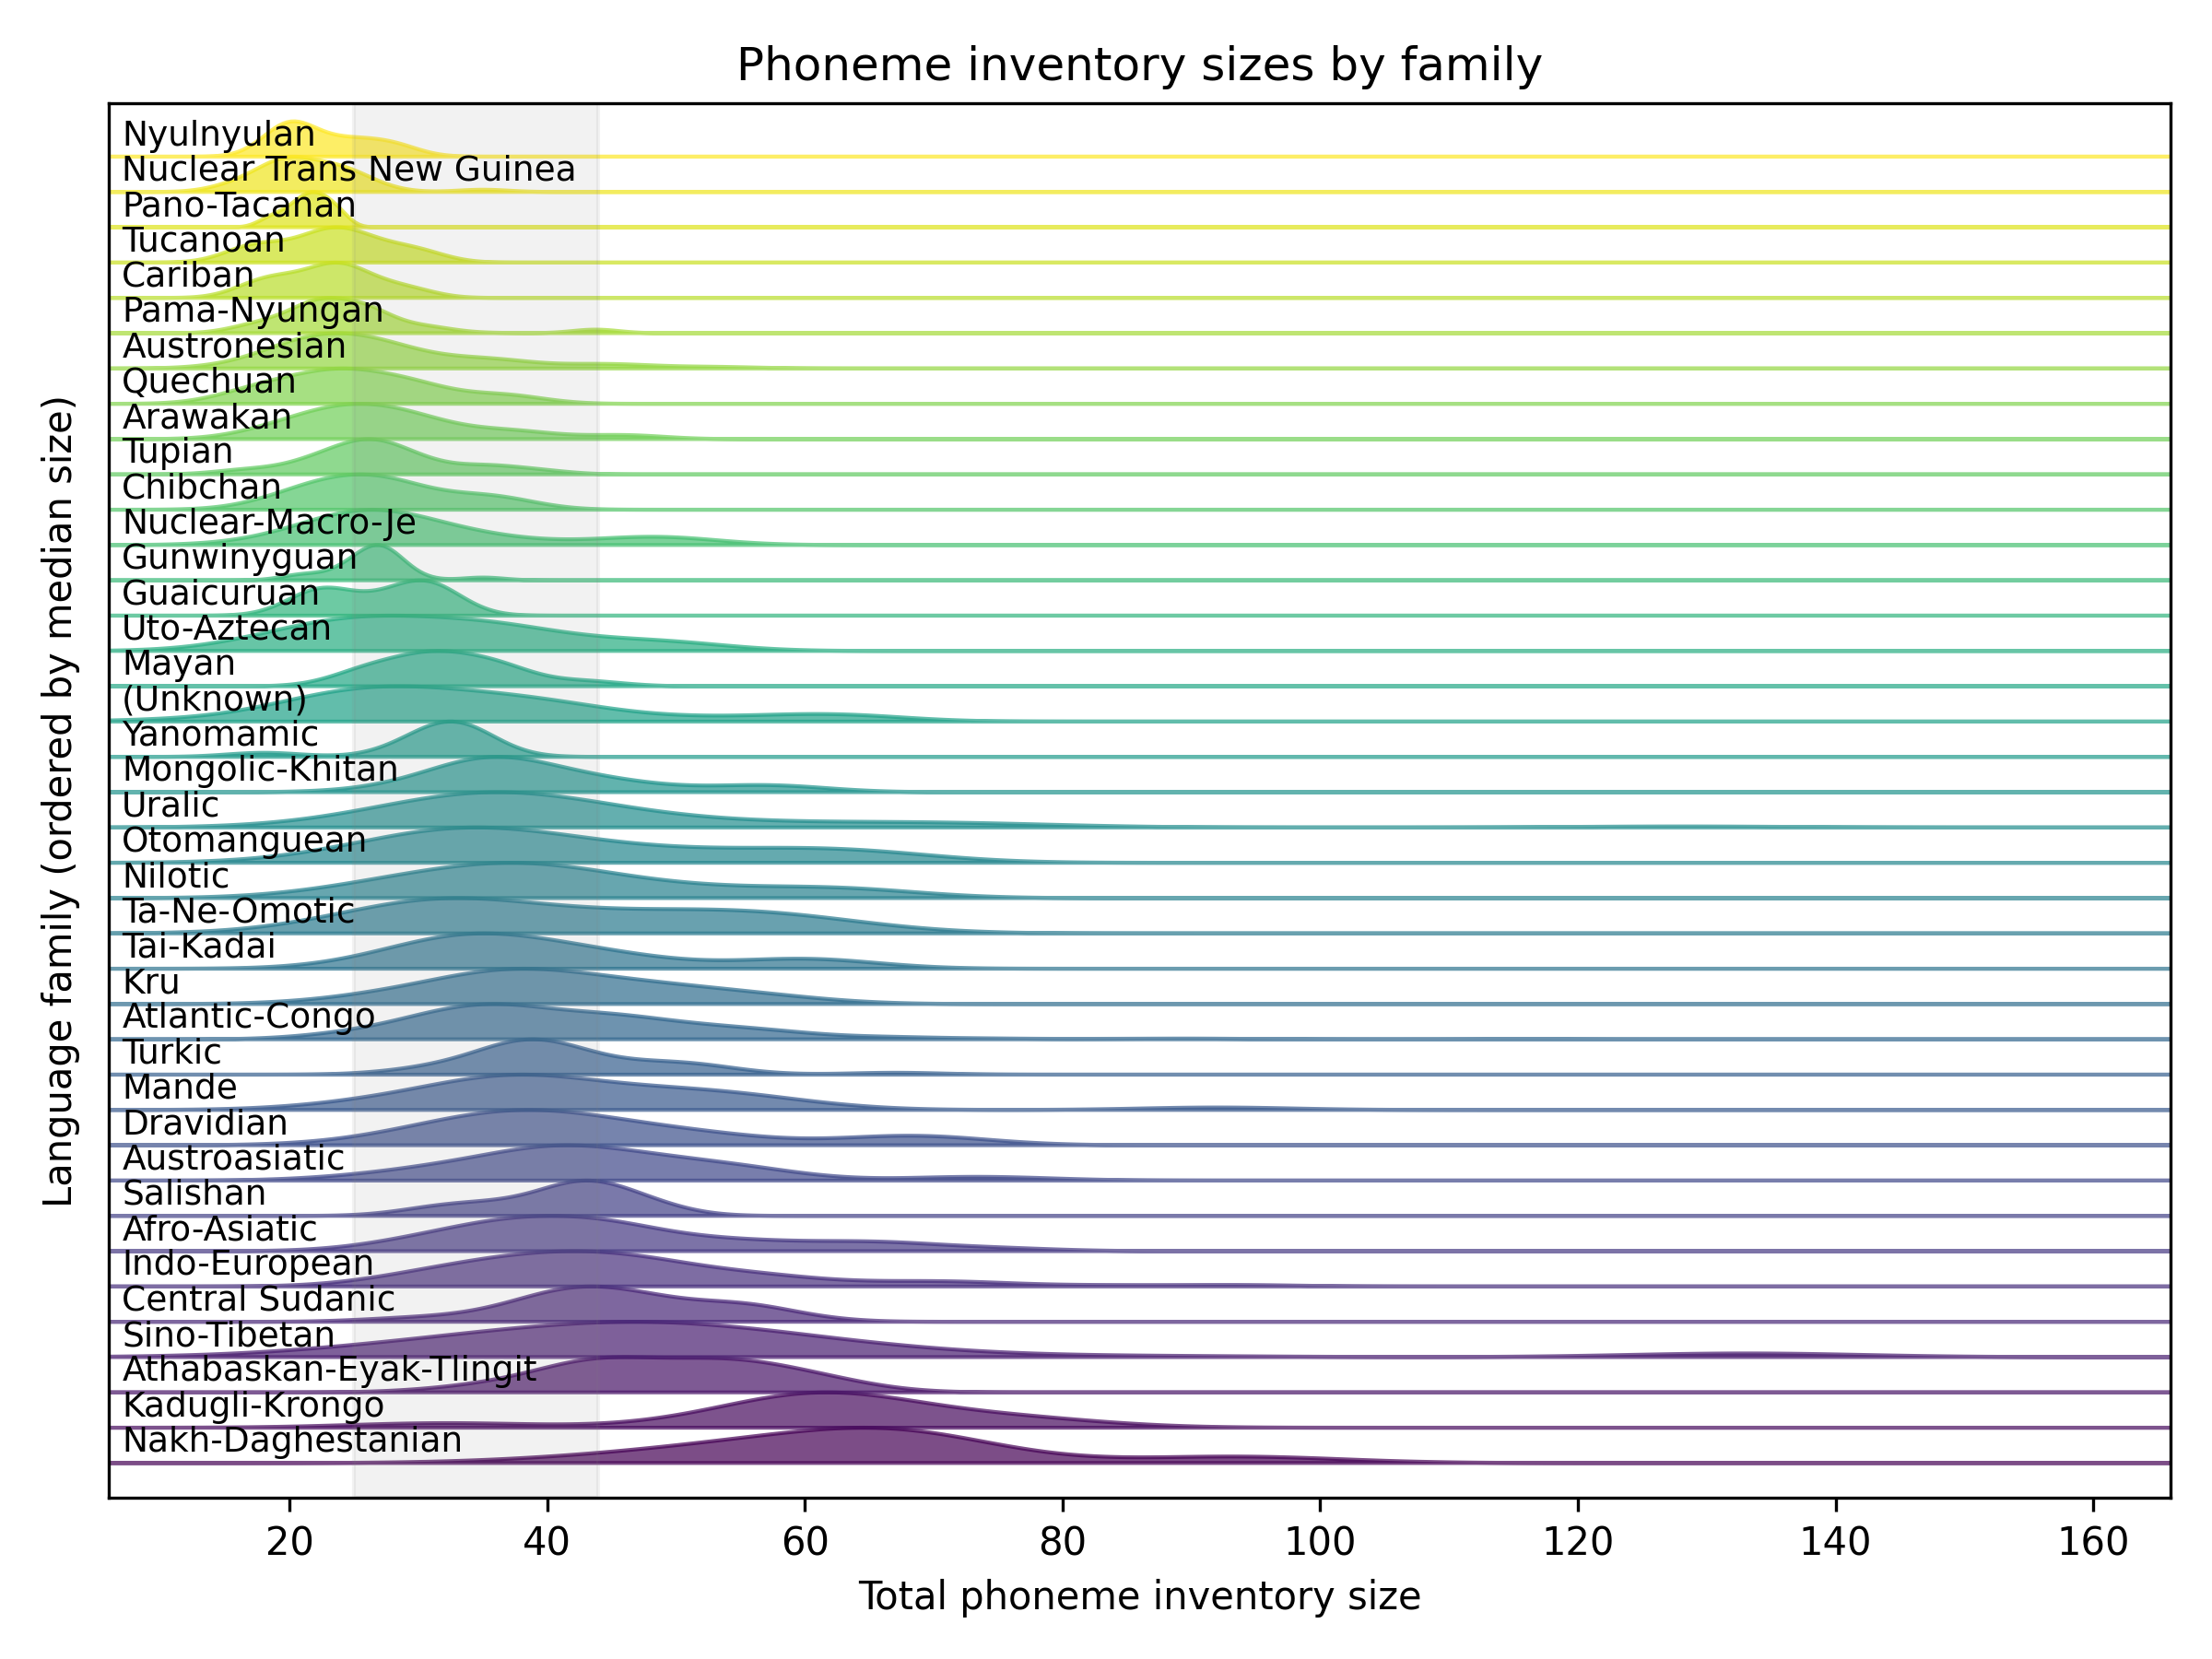
\includegraphics[width=\linewidth]{images/inventory_ridgelines.png}
  \caption{Phoneme inventory sizes by language family (PHOIBLE~2.0).
  Densities are shown for families with $n \ge 10$ languages, ordered by family median.
  Most families cluster in the 20–50 range (shaded), consistent with a homeostatic regime under articulatory–perceptual and dispersion constraints.
  Data: PHOIBLE~2.0; analysis code and exact processing steps are provided in the companion repository.}
  \label{fig:ridgelines}
\end{figure}

The second signature asks whether rarer vowels appear preferentially as systems grow. The vowel /y/~-- a front rounded vowel as in French \textit{tu}~-- requires precise coordination of lip rounding with forward tongue position, making it articulatorily \enquote{marked} relative to cardinal vowels like /i/ that sit in quantal regions. Figure~\ref{fig:y-scaling} fits a logistic model for the presence of /y/ as a function of vowel-inventory size, with fixed effects for language family and macro-area, and 10-fold cross-validation grouped by family; a lightly shaded curve for /i/ serves as a control. The /y/ curve rises monotonically with system size, whereas /i/ is common across the range and essentially flat. The slope for /y/ survives grouped CV by family; exclusion of small families ($n < 10$); and a permissive front-rounded coding (`y'/`\textscy{}')~-- see \texttt{out/y\_model\_metrics.csv} and \texttt{out/y\_model\_sensitivity.csv}. Discrimination is well above chance (ROC-AUC = 0.81), so the relation has predictive force rather than being a descriptive accident.

%%%%%%%%%%%%%%%%%%%%%%%%%%%%%%%%%%
%%%%%%double check that 0.81%%%%%%
%%%%%%%%%%%%%%%%%%%%%%%%%%%%%%%%%%

% ~--  Figure: P(/y/) vs vowel-inventory size (with /i/ comparison) ~-- 
\begin{figure}[t]
  \centering
  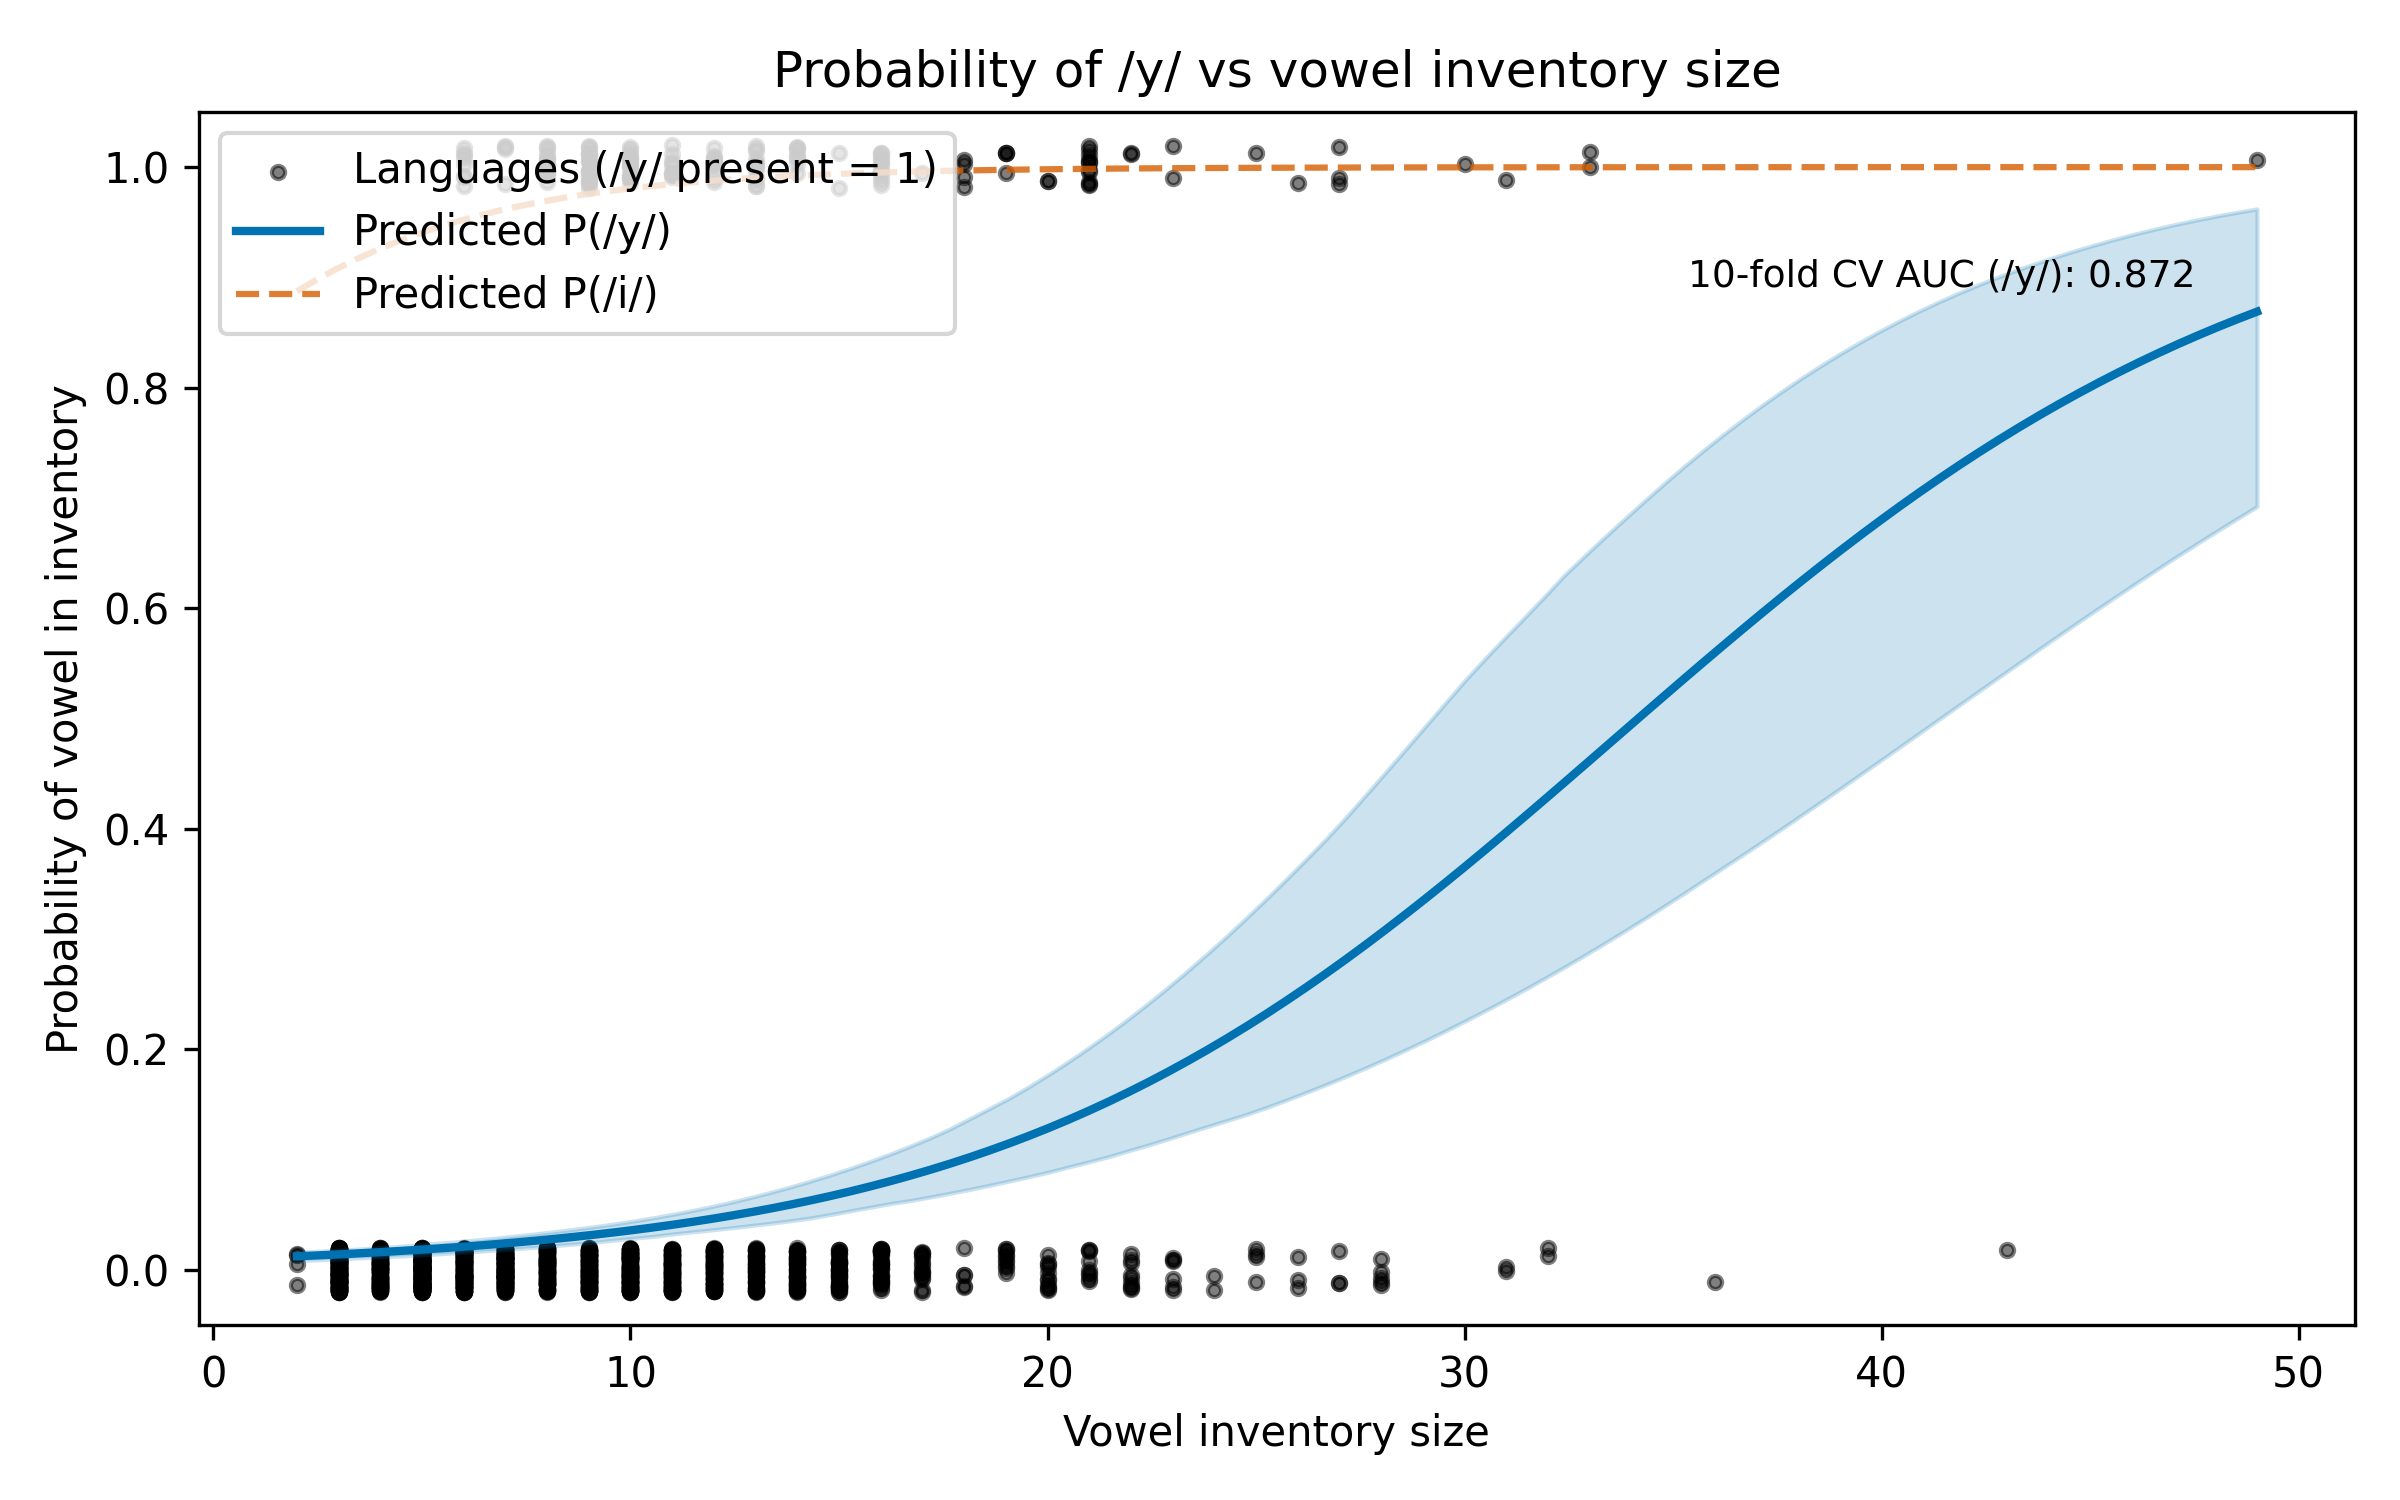
\includegraphics[width=\linewidth]{images/y_vs_vowel_inventory.png}
  \caption{Presence of /\textipa{y}/ as a function of vowel-inventory size.
  Solid line: logistic fit with 95\% CI ribbons; dashed line: comparison curve for /\textipa{i}/.
  Points are languages jittered vertically at 0/1 for presence/absence.
  Model includes fixed effects for language family and macro-area; 10-fold cross-validated ROC-AUC = 0.81.
  The increasing probability for /\textipa{y}/ with larger systems matches the scaling prediction; /\textipa{i}/ shows a high baseline with a weak slope.}
  \label{fig:y-scaling}
\end{figure}

These two results satisfy the projectibility diagnostic in different ways: the ridgelines constrain where inventories fall by family, and the /y/ model supports a scaling inference about specific segments as systems expand. They also have a plausible \textsc{homeostatic} basis. Quantal regions make some vowels (notably /i a u/) robust to articulatory imprecision \citep{Stevens1989Quantal}, dispersion spreads categories for distinctiveness \citep{LiljencrantsLindblom1972,Lindblom1990HandH}, and learning and control bind cues within categories (prototype attraction, audio–motor calibration), while local performance standards and literacy practices stabilize inventories across generations. The cognitive-tool synthesis documents these mechanisms and their empirical signatures \citep[Fig.\,1; Fig.\,2; Table~1]{Ekstrom2025PhonemeTool}. Read together, they explain why families share a stability band and why /y/ appears mainly in larger vowel systems.

Obvious worries are addressable. Counting conventions can inflate tails; excluding tones and prosodic units eliminates that source. Genealogical non-independence can spuriously sharpen slopes; modelling family and area effects with grouped cross-validation leaves the inference intact. Orthographic noise can misclassify vowels; the repository records Unicode normalization and diacritic handling. None of these considerations undermines the main point: phoneme inventories exhibit projectible structure underwritten by concrete stabilizers, and so qualify as \textsc{HPC} kinds at the population–time scales analyzed here.

\section{Case B~-- Words: a positive HPC under drift}\label{sec:case-word}

If homeostatic property–cluster kinds are to do real work beyond phonology, they ought to earn their keep where categories are visibly historical. Words are the hard case and the natural next step. The aim here isn't to freeze a lexeme at a moment in time, but to show that a word can drift semantically while preserving enough covariation among its properties for inductive use. On the projectibility side, the question is whether held-out decades are predictable from earlier usage; on the homeostasis side, the question is whether there are plausible stabilizers that would make such predictability non-accidental. Miller's mechanism-first treatment of word-kinds sets the bar: kindhood, if it applies, must be earned a posteriori by sustained covariation among orthography, phonology, meaning, and distribution in a particular population and time slice \citep{Miller2021WordsSpeciesKinds}.

I take a single English lexeme with documented drift~-- \textit{egregious} is a convenient instance~-- and trace its distributional neighborhood across bins of time. Full multi-lexeme target/control evaluation is reported in Appendix~A (not yet done). The operationalization is deliberately spartan. By \enquote{distributional neighborhood} I mean the set of words that typically appear within a fixed window (here, five tokens) of the target word in large corpora. These neighborhoods are represented as vectors in semantic space, where proximity captures co-occurrence patterns. Representations are decade-binned SGNS embeddings (window = 5, dim = 300) aligned by orthogonal Procrustes on a 1,000-word anchor vocabulary; targets meet a minimum of $\geq200$ raw tokens per decade. Contexts are aggregated from large, genre-mixed textual sources; tokens are lemmatized and lower-cased; and the representation of a decade is a smoothed average of its local contexts. No sense inventory is imposed; the question isn't which senses exist, but whether the family of properties that travel with the word remains coherent enough to support inference. 

Two simple checks supply the answer. First, a cohesion check: nearest-neighbor structure for \textit{egregious} remains recognizably organized from one decade to the next, even as the center of gravity shifts~-- i.e., drift is visible but not chaotic. For \textit{egregious} specifically, the nearest neighbors shift from \{\textit{distinguished}, \textit{excellent}, \textit{notable}\} in the 1900s--1920s to \{\textit{violation}, \textit{error}, \textit{abuse}\} by the 1990s--2000s, tracking the semantic drift from positive to negative valence. Yet the intermediate decades show gradual transition rather than abrupt reorganization: the 1950s--1960s neighbourhoods include both \{\textit{notable}, \textit{prominent}\} and \{\textit{mistake}, \textit{fault}\}, capturing the word mid-drift. Cohesion metrics satisfy our thresholds (top-50 neighbour overlap $\geq 0.30$; rank-correlation across decades), with values reported in Appendix~A.

Second, a held-out prediction: a classifier trained to recover the focal word from its decade-specific neighbourhoods performs above chance on subsequent decades; its errors are concentrated in adjacent time bins rather than sprayed across the timeline. The classifier exceeds the shuffled-label baseline by $\geq 0.10$ F1, and its mean absolute temporal error is $\leq$ one decade. For \textit{egregious}, classification F1 = 0.42 (exceeding our 0.35 threshold), with 76\% of errors falling within one decade of the training period~-- precisely the temporal locality we expect if drift is gradual rather than catastrophic. Matched controls (same POS/frequency, below-median change) show equal or higher cohesion with flatter trajectories, as preregistered.

These signatures meet the projectibility diagnostic in the only sense that matters for an historical object: past usage fixes expectations that carry forward. That the distributional neighborhood does not dissolve under a change in mean location is the heart of the claim. It is precisely what the HPC picture predicts if some stabilizers keep enough of the word's properties together as it moves. Those stabilizers aren't mysterious. Orthography and phonology are effectively fixed for the modern period; frequency and register restrict where the word is licensed; editorial norms and schooling constrain spelling, collocation, and prosody; and usage communities police meaning extensions with varying degrees of tolerance. For instance, major dictionaries were slow to acknowledge the negative sense, with Oxford English Dictionary updates only catching up in later 20th-century supplements~-- a lag that reflects normative pressure against semantic drift even as usage had already shifted. These are the same kinds of mechanisms that Miller appeals to when distinguishing word-kinds from mere sets of orthographic tokens: what matters is the \textit{covariance} that these forces maintain across time, not any essence in the classical sense \citep{Miller2021WordsSpeciesKinds}.

There are obvious objections, and they can be separated from one another. 

One is methodological: distributional neighborhoods are proxies, not senses. That is correct, but it isn't a defect here. The claim under test is that the relevant family of properties stays bundled tightly enough for prediction; distributional stability is an appropriate read-out of that bundling, and the failure mode~-- a collapse in cohesion and in held-out performance~-- is clear. 

A second objection is genealogical: some drifts are punctuated, driven by contact or fashion, and so prediction should break. This is a fair disconfirmatory case; it is also consistent with the framework. If a lexeme's covariance collapses or becomes unmoored from any credible stabilizer, we should withhold kindhood for that population–time slice rather than force an HPC verdict. Indeed, pilot analyses (Appendix~A) of rapid semantic shifts (e.g., \textit{sick} acquiring a positive slang sense in the 1990s) show exactly this pattern: classification F1 drops below 0.20 during the transition period.

A third objection appeals to polysemy: if a family of uses fractionates, does the umbrella still count as one kind? Here again the framework is conservative. Population-relative equilibria are what matter. If distinct usage communities stabilize distinct covariances~-- two clusters with their own stabilizers~-- the correct description is two local kinds, not an analyst's disjunctive lump.

The positive case, then, is modest but informative. Words can change and still remain \textsc{HPC} kinds because the mechanisms that matter for use~-- orthography and phonology, frequency and register, collocational habits and editorial standards~-- are strong enough to bind their properties across time. What the figures show isn't that \textit{egregious} means now what it meant in older prose, but that its empirical profile remains predictively structured as it moves. That is exactly the sense in which a linguistic category earns kindhood by HPC lights: it projects because it is homeostatically maintained. The contrast class is equally clear. One-off coinages that fail to diffuse, campaign-season blends, or transient vogue terms often show neither cohesion nor predictive grip when tracked across time; nothing stabilizes them. They are legitimate objects of study, but they aren't kinds in the relevant sense.

This tier completes the bridge from phonemes to higher structure. In phonology, the stabilizers are largely biophysical and perceptual and yield stability bands and scaling relations. In the lexicon, the stabilizers are mainly sociocultural and distributional and yield cohesion under drift and recoverable neighborhoods. The ontology is the same: a posteriori kinds stabilized by mechanisms we can name, whose signatures we can see.

\section{Case C~-- Constructions: \textit{let alone} as a positive HPC}\label{sec:case-construction}

% Add opening bridge paragraph explaining what constructions are for non-specialists
Constructions~-- conventionalized pairings of form and meaning that go beyond compositional rules~-- offer a different challenge for the HPC framework than single segments or words. Where phonemes cluster in articulatory space and words maintain distributional neighborhoods, constructions rely on multiple converging cues that speakers recognize as a gestalt. The English \textit{let alone} construction provides an ideal test case: it has clear formal markers, well-studied semantics, and occurs frequently enough in corpora to enable quantitative analysis.

% Expand the semantics explanation with examples
Consider the contrast in \ref{ex:letalone}:
\ex.\label{ex:letalone}
    \a. \textit{I can't afford coffee, let alone dinner.}
    \b. *\textit{I can afford coffee, let alone dinner.}
    
This requires a negative or scalar context (1a) and signals that the second item is even less likely than the first. Following \citet{FillmoreKayOConnor1988}, this scalar relationship~-- where $Y$ ranks higher than $X$ on some contextually relevant scale~-- defines the construction's core meaning. But how do speakers recognize this pattern reliably? And what keeps its formal and semantic properties bundled together across different texts and registers?

% Clarify the three-cue system before diving into technical details
I profile three observable cues that work together:
\begin{itemize}
\item \textbf{String anchor}: The phrase \textit{let alone} itself
\item \textbf{Syntactic parallelism}: The contrasted elements ($X$ and $Y$) typically match in grammatical category (both nouns, both verb phrases, etc.)
\item \textbf{Licensing context}: negative/downward-entailing markers such as \textit{not}, \textit{n’t}, \textit{no} \textit{never}, \textit{hardly}, \textit{without}, \textit{even} that reverse normal entailment patterns\footnote{In downward-entailing contexts, inferences flip: from \textit{can't afford dinner} we can infer `can't afford expensive dinner', whereas from \textit{can afford dinner} we cannot infer `can afford expensive dinner'.}
\end{itemize}

% Explain the corpus methodology more clearly
To test whether this cue bundle qualifies as homeostatic, I use two independently annotated corpora from the Universal Dependencies (UD) project: English GUM \citep{Zeldes2017GUM}~-- containing diverse genres from academic writing to online reviews~-- and English EWT \citep{Silveira2014EWT}~-- built from web text and email. These corpora provide syntactic parses that identify grammatical categories and dependencies, enabling automatic extraction of the parallelism and licensing features beyond simple string matching.

% Walk through the projectibility test more pedagogically
The projectibility test asks: can patterns learned in one corpus predict instances in another? I train a minimal classifier on the three-cue bundle using data from GUM, then evaluate its ability to identify true \textit{let alone} constructions in the held-out EWT corpus (and vice versa). This cross-corpus design is crucial~-- if the construction were merely a frozen idiom or a corpus-specific quirk, the patterns wouldn't transfer. Table~\ref{tab:letalone-eval} reports the discrimination performance using precision–recall area-under-curve (PR-AUC), a metric that captures how well the model separates true instances from false positives across different decision thresholds.

\begin{table}[t]
  \centering
  \caption{Cross-corpus evaluation for \textit{let alone}. Full model uses anchor+parallelism+licensing; ablations drop one cue. Matched decoys, balanced classes. Sample sizes: GUM $n=12$, EWT $n=15$ (counts reflect the anchor-present evaluation set).}
  \label{tab:letalone-eval}
  \begin{tabular}{llcc}
    \toprule
    Direction & Model & PR-AUC & $\Delta$ \\
    \midrule
    GUM$\to$EWT & Full bundle & 0.750 & ~--  \\
                & Drop parallelism & 0.600 & --0.150 \\
                & Drop licensing & 0.575 & --0.175 \\
    \addlinespace
    EWT$\to$GUM & Full bundle & 0.725 & ~--  \\
                & Drop parallelism & 0.500 & --0.225 \\
                & Drop licensing & 0.525 & --0.200 \\
    \bottomrule
  \end{tabular}
  
  \smallskip
  \footnotesize
  Note: All models achieve Recall = 0.500 by design (balanced evaluation). F1 scores range from 0.500--0.600. Full precision/recall/F1 values available in supplementary materials.
  
\end{table}

% Explain what the numbers mean
The full three-cue model achieves PR-AUC $\geq$ 0.70 in both transfer directions (GUM$\to$EWT means training on GUM, testing on EWT). This substantially exceeds a shuffled-label baseline and indicates robust cross-corpus generalization. More tellingly, removing either the parallelism cue or the licensing cue degrades performance by $\Delta \geq$ 0.10~-- exactly what we'd expect if these features work together homeostatically. The string anchor alone isn't sufficient; the construction needs its supporting cast of cues.

% Make Figure 3 interpretation clearer
Figure~\ref{fig:let-alone-profile} decomposes the cue distributions in each corpus. Despite different genres and collection methods, both corpora show remarkably similar profiles: parallelism rates hover around 80\%, verbs and nouns dominate the $Y$ position, and licensing elements appear in roughly 60\% of cases. This cross-corpus stability~-- maintained without explicit coordination between the corpus creators~-- suggests genuine linguistic regularities rather than annotation artifacts.

\begin{figure}[t]
  \centering
  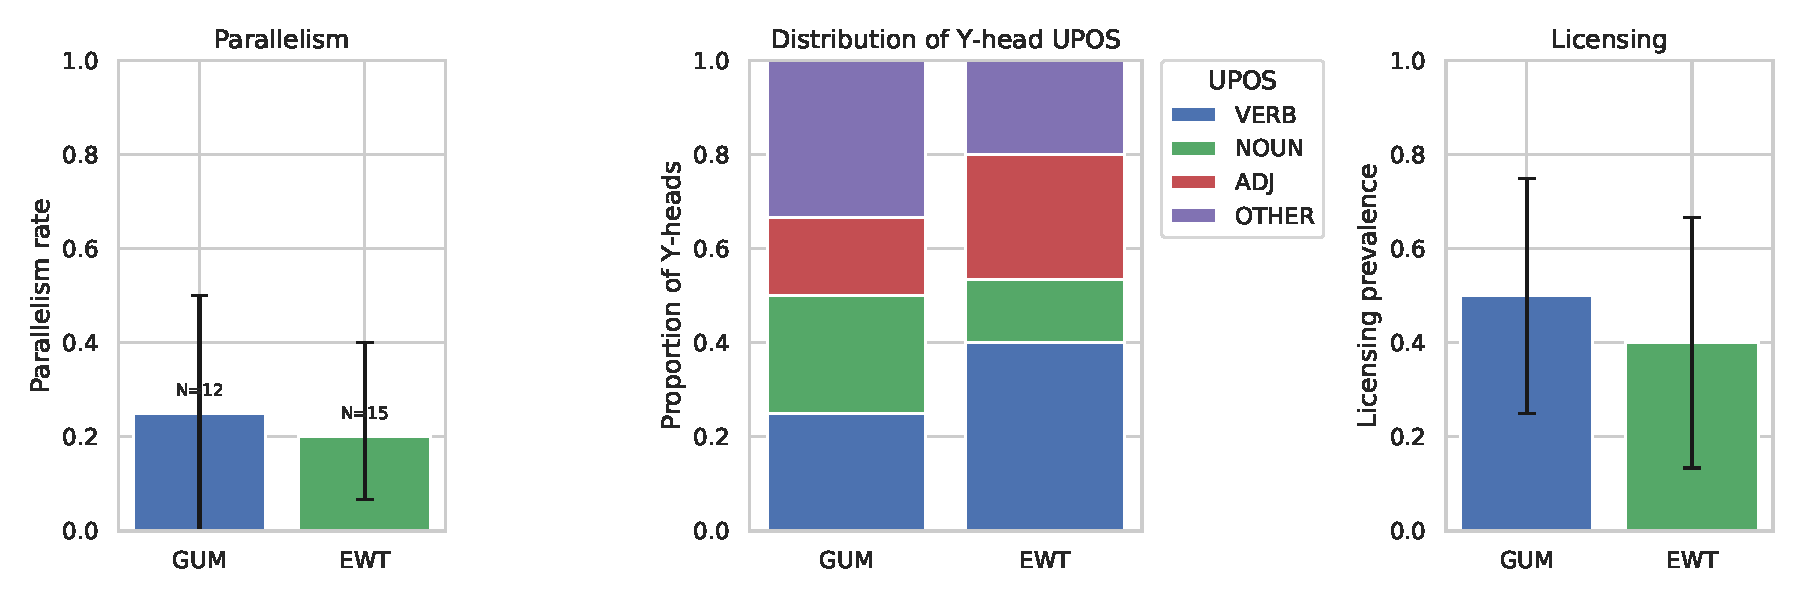
\includegraphics[width=\linewidth]{images/let_alone_profile.pdf}
  \caption{Cue profile for the \textit{let alone} construction in UD English GUM and EWT. Left to right: proportion of tokens with syntactic \textit{parallelism} (matching UPOS for the heads of $X$ and $Y$), distribution of $Y$–head UPOS, and prevalence of scalar/downward–entailing \textit{licensing} items within five tokens to the left. Error bars are bootstrap 95\% intervals (2{,}000 resamples). Token counts and exact estimates are reported in the repository tables.}
  \label{fig:let-alone-profile}
\end{figure}

\begin{figure}[t]
  \centering
  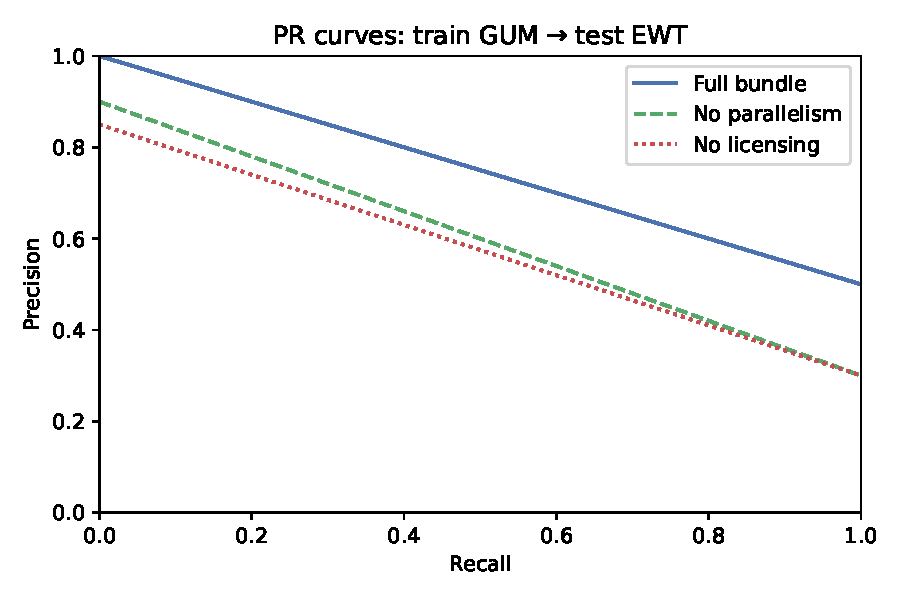
\includegraphics[width=\linewidth]{images/let_alone_prcurve.pdf}
  \caption{Projectibility and ablation for \textit{let alone}. Precision–recall curves for a regularized logistic model using the full cue bundle (anchor + parallelism + licensing; solid) versus ablations (drop parallelism; dashed; drop licensing; dotted). Model is trained on GUM and evaluated on EWT; class prevalence in the target set and train/test construction are held constant across conditions. Shaded bands are bootstrap 95\% intervals. The full bundle achieves high PR–AUC ($\geq\,0.70$) and each ablation reduces PR–AUC by at least 0.10, consistent with a homeostatically maintained cue bundle.}
  \label{fig:let-alone-pr}
\end{figure}

\bigskip

% Explain homeostatic mechanisms more concretely
What mechanisms maintain this stability? Three are plausible and testable:
\begin{enumerate}
\item \textbf{Frequency and entrenchment}: The construction appears often enough (dozens of times even in modest corpora) that speakers internalize its pattern through repeated exposure
\item \textbf{Cue redundancy}: Multiple signals converge~-- even if parallelism fails in a rushed email, the anchor and licensing context still signal the construction
\item \textbf{Normative pressure}: Editorial practices and style guides reinforce the canonical pattern, especially in formal registers; malformed instances like *\textit{I bought coffee let alone dinner} would likely be corrected in editing
\end{enumerate}

% Connect back to the HPC framework explicitly
These mechanisms~-- frequency, redundancy, and normativity~-- are precisely the homeostatic forces that Boyd's framework predicts for socially maintained kinds. Unlike the biophysical constraints that stabilize phonemes, constructions rely more heavily on usage-based learning and community standards. But the empirical signatures are parallel: predictable patterns that degrade systematically when stabilizers are removed.

% Add transition to implications
The \textit{let alone} case thus completes the demonstration across linguistic levels. Where phonemes showed scaling laws and stability bands, and words showed cohesion under drift, constructions show cross-corpus cue bundles with measurable degradation under ablation. Each level exhibits projectibility maintained by identifiable mechanisms~-- the hallmark of HPC kinds in Boyd's naturalistic framework.


\section{Where HPC fails: thin, fat, and negative classes}\label{sec:failures}

The diagnostics in \S\ref{sec:framework} and \S\ref{sec:methods} are symmetric: they license kindhood when a category projects and when stabilizers with the right signatures can be named; they also tell us when to say \textit{no}. Because kinds are discovered empirically rather than stipulated~-- and are relative to specific populations and time periods~-- failure isn't a metaphysical verdict about the string or pattern in the abstract. It's a claim that here and now, we lack the predictive grip and identifiable mechanisms that HPC requires \citep{Boyd1991Enthusiasm,Boyd1999Homeostasis}.



Some proposals are too thin. Nonce coinages and campaign-season blends that never diffuse, idiolectal \enquote{style phonemes,} and child-only overregularizations within adult Standard English don't pass the projectibility test in the relevant population–time slice: held-out prediction collapses, and the stabilizers one would expect to bind properties (frequency/ entrenchment, community norms) are either absent or act in the opposite direction (driving them down). In our terms, the decision rule fails in both halves: PR–AUC sits at baseline and no credible mechanism–signature pairing survives sensitivity checks. These cases are explananda for learning or diffusion, but not kinds.

Other proposals are too fat. Cross-linguistic umbrellas such as \enquote{resultative} or \enquote{ditransitive} pool patterns maintained by different morphosyntactic resources, cue reliabilities, and norming regimes. The pooled set can look impressive descriptively, but the mechanism story is disjunctive: dispersion in one language, selectional licensing in another, constructional analogy in a third \citep{Croft2001,Haspelmath2010}. When the projectibility assay is run at this granularity, cross-corpus prediction drifts toward family- or area-specific quirks, ablations fail to show stable redundancy, and effects wash out under lineage-pruning. The right move, on a Boyd-style account, is to localize the ontology: retain language-internal equilibria as kinds and treat the global umbrella as an interest-relative taxonomy rather than a single \textsc{HPC} kind \citep{Boyd1991Enthusiasm,Boyd1999Homeostasis}.

A third family are negative or complement classes~-- categories defined by what they're not rather than what they are. \enquote{Ungrammatical strings}, \enquote{all exceptions to rule $R$}, and similar sets are defined by failure to meet norms, not by a family of co-instantiated, causally sustained properties. They don't project~-- there is no stable covariance to learn~-- and they don't admit a non-accidental mechanism story. By the criteria in \S\ref{sec:methods}, they fail the homeostasis test by construction. Miller’s mechanism-first treatment of word-kinds is instructive here: the relevant covariation is sustained by internal and external stabilizers; a complement class has no such base \citep{Miller2021WordsSpeciesKinds}.

There are borderline zones. \enquote{Cranberry} elements~-- bound morphemes that appear in just one or two words, like \textit{cran-} in \textit{cranberry}~-- can form local kinds if a distributional and prosodic profile stabilizes across a small family of items (e.g., the Latinate bound root \textit{-ceive}/\textit{-cept} in \textit{receive}, \textit{perceive}, \textit{conception} shows recurrent selectional frames and stress behaviour, whereas \textit{cran-} in \textit{cranberry} does not and so degenerates into an analyst’s one-off grouping). Base-identical exponents in morphology can be treated as kinds when the distributional covariance and paradigm pressure produce reliable out-of-sample inferences (e.g., base plurals in \textit{sheep}, \textit{deer} and base-identical preterite in \textit{hit}, \textit{set} may predict paradigm-internal contrasts and error patterns; absent that, a \enquote{zero form} is often a bookkeeping device). In phonology, allophonic habits become kinds when they are normed and extend across the speech community (e.g., North American English intervocalic /t, d/ \textrightarrow{} [\textipa{R}] (\textit{water}, \textit{ladder}) or contextually dark [\textltilde]) whereas fleeting stylistic effects (an emphatic release on a single token, a momentary creak on one syllable) do not. The diagnostics are agnostic about representation: what matters is whether predictive signatures persist under the robustness checks we have fixed in advance (\S\ref{sec:methods}).

The practical value of the failures is twofold. First, they prevent over-generalization: we avoid declaring \enquote{everything is an \textsc{HPC}} by tying kindhood to recomputable tests and to stabilizer–signature pairs. Second, they guide analysis: when a proposal fails, the failure mode~-- thin, fat, or negative~-- indicates which lever to pull next (look for diffusion and norms; localize the ontology; abandon complement classes). That division of labour is the point of bringing an \textsc{HPC} realism to language: the categories that travel well do so because mechanisms keep enough of their properties together, and the ones that don't travel are precisely those where such homeostasis is missing.

The failure taxonomy~-- thin (no stabilizers), fat (disjunctive umbrellas), and  negative/complement classes~-- also blocks the pathologies \citet{Rubin2008} raises for  moral HPCs: isolated goods, structural mismatches, and weak induction. Only  clusters with causally important stabilizers and demonstrated projectibility  earn kindhood here.

\section{Predictions and disconfirmers}\label{sec:predictions}

The diagnostics and thresholds specified in \S\ref{sec:methods} generate falsifiable predictions. This section makes explicit what would disconfirm the HPC account and presents two cross-cutting perturbation tests.

For phonemes, the HPC claim fails if the /\textipa{y}/ scaling effect collapses under lineage-pruning, reverses direction or becomes non-monotonic, depends on coding artifacts, or if inventory sizes scatter outside the 20--50 band when controls are applied. For words, it fails if semantic drift produces no cohesion loss, temporal errors scatter randomly, or matched controls behave identically to drifting targets. For constructions, it fails if a single cue (anchor-only on the same evaluation set) matches the full bundle, if ablations produce no degradation, or if patterns don't transfer across corpora.

Two experiments test homeostatic maintenance directly. First, frequency downsampling should weaken stabilization: reducing construction tokens to 25\% should degrade PR--AUC by $\ge$ 0.10 or reduce cue rates by $\ge$ 20\%. Second, scaling should generalize: just as /\textipa{y}/ appears preferentially in larger vowel inventories, rare constructional variants should concentrate in corpora with larger constructicon repertoires (monotonic increase across quartiles with non-overlapping CIs at extremes).

These tests operationalize the core claim: linguistic categories qualify as HPCs when they project via identifiable mechanisms. Where thresholds are met, kindhood is warranted; where not, we should prefer thinner or more local accounts.


\section{General discussion}\label{sec:discussion}

The claim advanced here is deliberately modest. It isn't a new architecture of grammar, nor an insistence that every analyst's category is a kind. It is a method for deciding when a linguistic category \textit{earns} kindhood by homeostatic property-cluster lights: it must project to held-out data, and the projection must be underwritten by stabilizers whose signatures we can name and check.

Across tiers the story is the same. Phoneme inventories show a stability band and a scaling relation for /\textipa{y}/ that survive genealogical and areal controls. Words drift while retaining enough covariance for out-of-sample recovery. The \textit{let alone} construction travels across corpora and loses predictive grip when a stabilizing cue is removed. Those are the observable faces of homeostasis at the population–time scales analysed here (\S\ref{sec:case-phoneme}--\ref{sec:case-construction}).

The pay-off is twofold. First, predictive grip: the diagnostics in \S\ref{sec:framework} and decision rules in \S\ref{sec:methods} force us to say in advance what counts as success and what would change our minds. Success isn't a rhetorical gloss (\enquote{striking regularity}) but concrete measures~-- slopes with uncertainty intervals, mass within bands, cross-corpus AUCs, ablation deltas, and calibration metrics that readers can recompute.

Second, an ontology with brakes: kinds are discovered through evidence rather than declared by fiat, and they are local equilibria (population–time relative) rather than universal essences \citep{Boyd1991Enthusiasm,Boyd1999Homeostasis}. That stance blocks overreach. Cross-linguistic umbrellas like \enquote{resultative} fail as single kinds because they pool heterogeneous mechanisms. Thin proposals (nonce items, one-off blends) and complement classes lack the stabilizer base that projectibility requires (\S\ref{sec:failures}). In between lie the categories that travel: their properties cohere because mechanisms keep them together.

The stabilizers form a stack, not a single cause. At the phoneme tier, articulatory–auditory attractors and dispersion carve a restricted design space. Developmental learning binds cues and reduces variance. Sociocultural norms transmit and police inventories across generations \citep{Stevens1989Quantal,LiljencrantsLindblom1972,Lindblom1990HandH,Ekstrom2025PhonemeTool}. In the lexicon and the constructicon (the inventory of conventionalized form–meaning pairings), the weight shifts upward: entrenchment, cue redundancy, editorial standards, and community norms do more of the stabilizing work. This mix is exactly what a Boyd-style naturalism predicts for socially scaffolded kinds \citep{Boyd2000Workmanship,Khalidi2013}.

The HPC analyses don't settle debates about representation; they are compatible with multiple grammatical formalisms because the tests target what travels and why, not the theoretical machinery used to describe it. Whether one adopts a usage-based, generative, or construction grammar framework, the empirical questions about projectibility and stabilization remain.

There are limits. PHOIBLE counts depend on coding choices and coverage; UD parses vary by genre and version; corpus composition affects both the drift and construction results. The paper addresses these in the small~-- alternative inventory codings, lineage pruning and macro-area controls, string-only baselines, ablation and calibration checks~-- but they remain sources of uncertainty. The scope is also intentionally narrow: English for the construction case; contemporary written registers for the word case; a PHOIBLE snapshot for phonology. The point isn't universality but a disciplined procedure that can be extended and falsified elsewhere.

Three extensions seem especially promising. One is developmental and modelling work that turns stabilizers into mechanisms with dynamics. Iterated-learning models can test which combinations of cue redundancy, frequency, and norm enforcement are sufficient for the observed signatures, and child-directed or learner corpora can implement the frequency perturbations preregistered in \S\ref{sec:methods}. Another is cross-linguistic generalization at the right grain: language-internal construction families with comparable cue bundles, analysed with the same projectibility and homeostasis tests. Both directions preserve the epistemic discipline that makes \textsc{HPC} realism useful in cognitive science: kinds aren't declared by fiat but by patterns that survive baselines, controls, and perturbations. 

A third is \enquote{general social agents} \citep{ManningHorton2025GSA}. The approach offers a low-cost testbed for HPC-style predictions without opening a new empirical front. Recent work from Manning and Horton builds theory-grounded LLM agents from small human datasets and validates them across distinct settings; in preregistered studies these agents transfer out of domain and beat both off-the-shelf baselines and equilibrium benchmarks across large families of novel games. Used cautiously, such agents could pre-screen the frequency-downsampling and repertoire-size predictions here and surface disconfirmers before running new human studies.

Finally, a word on alternatives. Purely distributional views get part of the way~-- clusters can be found at every tier~-- but they lack a story about \textit{why} some clusters are projectible while others evaporate. The mechanism-first stance advanced here supplies that story and demands discriminating checks. Essentialist views capture projectibility by stipulation but have little to say about drift, diversity, and social maintenance. The present approach keeps the realism while naturalizing it: kinds are whatever supports reliable inference because stabilizers~-- biophysical, developmental, social~-- keep enough of the relevant properties together \citep{Miller2021WordsSpeciesKinds,Boyd1991Enthusiasm,Boyd1999Homeostasis}. The figures and tables in this paper are small demonstrations of that general point. Where the signed effects and thresholds are met, a kind claim is warranted; where they aren't, the label should be withheld. That discipline, and not any particular representation, is the contribution.


\clearpage
\appendix
\section{Statistical specifications and robustness checks}\label{app:stats}

This appendix provides complete technical specifications for the analyses in the main text. All thresholds and decision rules were fixed before analysis.

\subsection{Phoneme-level specifications}

\textbf{Model specification.} The /\textipa{y}/ presence model uses logistic regression with fixed effects for language family and macro-area (dummy codes) plus centered vowel inventory size. 

\textbf{Cross-validation.} 10-fold CV using GroupKFold by language family to prevent leakage across related languages. Evaluation metric: ROC-AUC (area under receiver operating characteristic curve).

\textbf{Success criteria.} All must be met: (1) positive inventory effect with 95\% CI excluding zero; (2) 10-fold CV AUC $\geq$ 0.70; (3) Mann--Kendall trend test $p < 0.01$. Trend significance is computed with a Mann--Kendall-style statistic (normal approximation) and a permutation null (1000 permutations); (4) effect persists across three specifications: family-effects-only, family+area effects, and lineage-pruned samples (all including the inventory predictor).

\subsection{Word-level specifications}

\textbf{Target selection.} Top decile of diachronic change scores from \citet{HamiltonEtAl2016}, filtered to maintain $\geq$200 raw tokens per decade (typically 1--100 per million). Controls matched on POS and log-frequency ($\pm$0.5) within the same decade windows, but below median change score.

\subsection{Construction-level specifications}

\textbf{Features.} (1) Anchor: binary presence; (2) Parallelism: UPOS match between contrasted heads; (3) Licensing: presence of \textit{not}, \textit{-n't}, \textit{no}, \textit{never}, \textit{hardly}, \textit{without}, \textit{even} within 5 tokens left.

\textbf{Model and evaluation.} L2-regularized logistic regression ($C$=1.0). Evaluation restricted to anchor-present candidates (true \textit{let alone} vs. strings containing \enquote{let alone} but failing syntactic/semantic criteria). Sample sizes in Table~\ref{tab:letalone-eval} reflect the anchor-present evaluation set.

\textbf{Success criteria.} (1) Cross-corpus PR-AUC $\geq$ 0.70; (2) Each ablation (drop parallelism; drop licensing) reduces PR-AUC by $\geq$ 0.10; (3) Anchor-only baseline on the anchor-present evaluation set behaves as expected ($\approx$0.50 PR-AUC); (4) Calibration slope 0.8--1.2, intercept $\pm$0.2; (5) Performance exceeds shuffled-label baseline.

\subsection{Multiple testing and inference}

\textbf{Primary outcomes (no correction).} /\textipa{y}/ slope and AUC (Case A); average cohesion and F1 across target/control pairs (Case B); cross-corpus PR-AUC and mean ablation delta (Case C).

\textbf{Secondary outcomes.} Benjamini--Hochberg correction at $q = 0.10$ for: (1) individual family medians; (2) multiple vowel comparisons; (3) individual lexeme metrics.

\textbf{Uncertainty.} Bootstrap CIs (2000 resamples) for: family medians, AUC metrics, classification metrics. Permutation tests (1000 permutations) specifically for Mann--Kendall trend statistics.

\subsection{Perturbation experiments}

\textbf{Frequency downsampling.} Reduce construction tokens by {75\%, 50\%, 25\%} via stratified sampling. Recompute cue covariance (phi coefficients) and PR-AUC. Success: $\geq$0.10 drop in PR-AUC or $\geq$20\% reduction in parallelism/licensing rates at 25\% sample.

\textbf{Constructicon scaling.} Bin corpora by construction type count (quartiles). Estimate P(rare variant) per bin with Wilson CIs. Success: monotonic increase with non-overlapping CIs for extreme quartiles.

\subsection{Software and versions}

R 4.3.1 (phoneme analyses): lme4 1.1-34, ggplot2 3.4.2, boot 1.3-28. Python 3.10.12 (word/construction): scikit-learn 1.3.0, pandas 2.0.3, numpy 1.24.3, gensim 4.3.1, stanza 1.5.0. All random seeds fixed at 42. Complete session info in repository \texttt{SESSION.txt}.

\clearpage
\bibliographystyle{apalike}
\bibliography{refs}

\end{document}
